\beginsong{Near to Banbridge Town}[txt={Cathal MacGarvey}, mel={Musik aus dem Irischen, 1726}, bo={242}, pfii={184}, pfiii={10}, siru={170}]

\beginverse
\endverse
\centering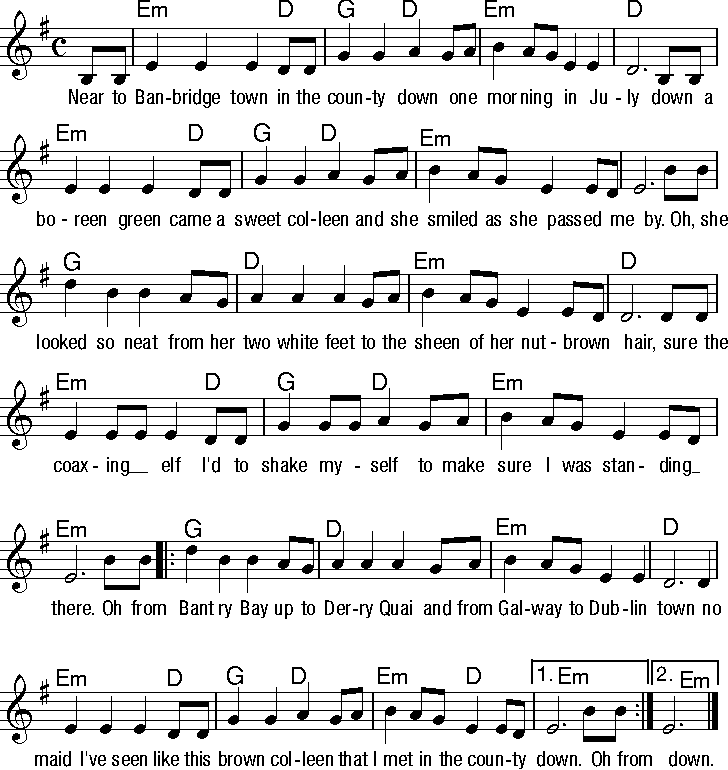
\includegraphics[width=1\textwidth]{Noten/Lied070.pdf}	

\beginverse
As she \[Em]onward sped, \[D]sure I \[G]scratched my \[D]head an I \[Em]looked with a feeling \[D]rare
And I \[Em]say, says I \[Dm]to a \[G]passer-\[D]by: 'Who's the \[Em]maid with the nut-\[D]brown \[Em]hair?'
He \[G]smiled at me and he \[D]says, says he: 'That's the \[Em]gem of Ireland's \[D]crown!
Young \[Em]Rosie McGann \[D]from the \[G]banks of the \[D]Bann, she's the \[Em]star of the Coun\[D]ty \[Em]Down.'
\endverse

\beginchorus
\lrep Oh, from \[G]Bantry Bay up to \[D]Derry Quay and from \[Em]Galway to Dublin \[D]Town,
No maid \[Em]I've seen \[D]like this \[G]brown col\[D]leen, that I \[Em]met in the Coun\[D]ty \[Em]Down. \rrep
\endchorus

\beginverse
At the ^harvest fair ^she'll be ^surely ^there, so I'll ^dress in my sunday ^clothes
With my ^shoes shone bright ^and my ^hat cocked ^right for a ^smile of my nut-^brown ^rose.
No ^pipe I'll smoke, no ^horse I'll yoke, till my ^plough is a rust-coloured ^brown,
Till a ^smiling bride ^by my ^own fire^side sits the ^star of the Coun^ty ^Down.
\endverse

\renewcommand{\everychorus}{\textnote{\bf Refrain (wdh.)}}
\beginchorus
\endchorus

\endsong

\beginscripture{}
Das Lied The Star of the County Down ist eine irische Ballade von Cathal Mac Garvey (1866-1927). Die Melodie ist weitaus älter und bereits im 1726 erschienen Buch ''Music for Allan Ramsay's Collection of Scots Songs'' von Alexander Stuart unter der Bezeichnung Gilderoy dokumentiert. Auf die gleiche Melodie gibt es zahlreiche weitere Lieder.
Das Lied wird vom Standpunkt eines jungen Mannes aus gesungen, der eine junge Frau namens Rose McCann trifft, die als ''Stern der Grafschaft Down'' bezeichnet wird.
\endscripture
